% Look!  A mock introduction

The introduction is one of the most important pieces of your thesis.  Here is a place for you to introduce the problem(s) on which you have worked and place them in the larger context of your field.  You should aim to ensure that this section is completely understandable to virtually anyone - and certainly anyone with a sophomore-level grasp of physics.  Presumably this will include references to the literature.

In addition to setting your work into context, a second good idea for your introduction is to give a short outline for what the rest of your thesis will discuss.  This is often done in the closing paragraph(s) of the introduction with sentences like ``In the following chapters \ldots " and ``Chapter 2 discusses \ldots"  Tremendous detail is not required in this outline, but rather just a brief road map for the rest of the document.

\section{A section}

The \texttt{\textbackslash section} tag will create a new section within a chapter.  Sections will be sequenced with digits following a decimal point in the table of contents, i.e. this is section 1.1.

\section{Another section}

This second section is, obviously, 1.2.

\subsection{A subsection}

Subsections are created using the \texttt{\textbackslash subsection} delineate smaller pieces of your document, and will appear after a second decimal point; this is subsection 1 of section 2 of chapter 1, i.e. 1.2.1.

\subsubsection{A subsubsection}

Subsubsections are still smaller sections.  By default, this is the finest subdivision of a chapter in \LaTeX, and they will \emph{not} appear in the table of contents.  

\subsection{A useful command}

\marginpar{This is a margin note.}
One command I often ask my students to use is \texttt{\textbackslash marginpar}, which can be used to create a margin note.  These are super helfpul if there's something to which you need to return later (say, after you've looked up a number), as notes in the margin are really easy to find quickly.  

\section{Some figures}

You will surely want to add figures to your thesis to help explain your ideas.  There are a number of different ways to include such things, but the most typical way would be to generate the figure in another piece of software (\texttt{MATLAB, Mathematica, Adobe Illustrator, \ldots} and simply include it in your \LaTeX ~code.  This will require use of the \emph{figure} environment.\footnote{there are many other possible environments to include figures, such as wrapfigure, but these will require including additional packages \ldots}  See this document's \LaTeX ~code for details . . .

% Here is the figure environment.  The [] after \begin{figure} are an optional argument that tells LaTeX where to try to place the figure.  If you do not include it then it will figure out the `best' place to put things on its own, but on occasion the choices it makes are a bit strange.  Even so, you should probably try to let it make the decisions whenever possible, and only come back to enforce new locations after you have essentially finished your document.  Otherwise you may find that your instructions are no longer appropriate if you add text elsewhere in the document that changes how things are alligned.  Anyhow, [h] instructs LaTeX to put th e figure `here', and adding an exclamation point [h!] means REALLY, PUT IT HERE.  [t] and [b] mean to put the figure at the top or bottom of a page, respectively.
\begin{figure}[h!]

%\centering centers the figure on the page.  This is convention.
\centering

% The \includegraphics command is the default way to include a figure.  The first optional argument in [] brackets defines how large the figure should be on the page.  This can be defined in inches, centimeters, or as a fraction of the \textwidth.  Then, in the curly {} braces you will put the file name for the figure.  Here it has been stored in a subfolder entitled Figures.  You are encouraged to give your figures descriptive file names, as this will help future students to figure out what figure corresponds to which file without having to read your LaTeX code.  
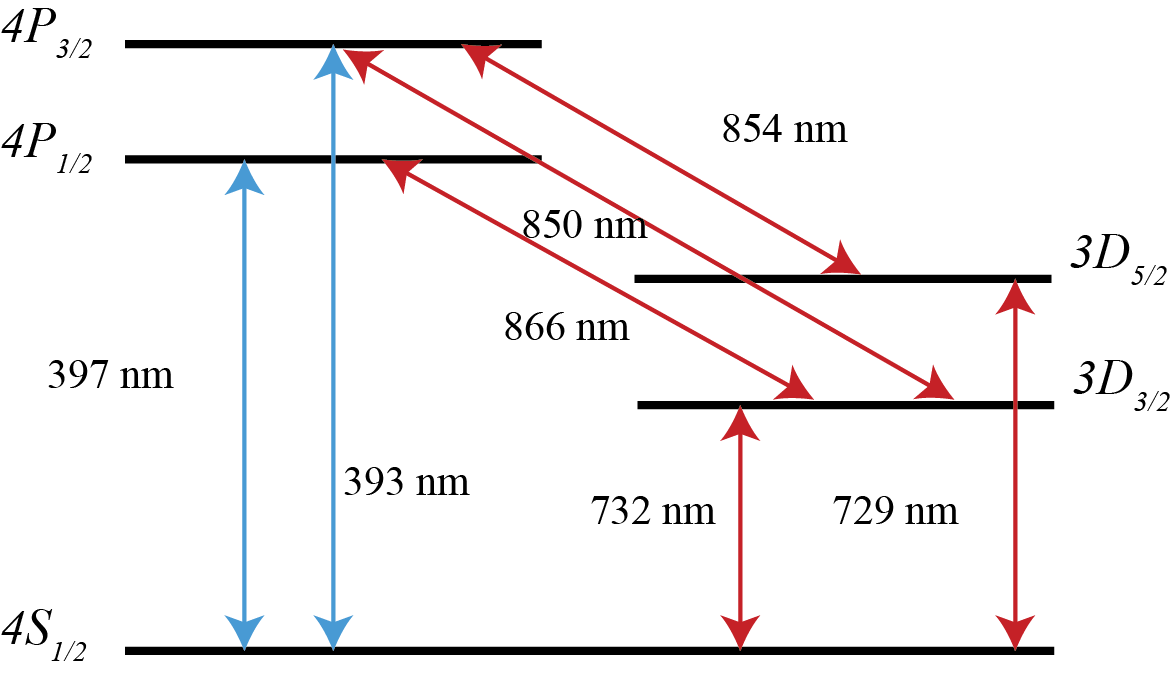
\includegraphics[width=.8\textwidth]{Chapters/Figures/calcium_levels_1-1.PNG}

%\caption will create a figure caption.  Putting an asterisk after it (as in \caption* ) will cause the caption to not be numbered and to not appear in the list of figures.  The [] argument is optional but recommended; this is the short-form caption which will appear in the list of figures.  The {} argument is required, and gives the full caption which will appear in the main text.  The first few words of this caption will be used in the list of figures if no [] form is given.  
\caption[Short-form caption]{Long-form caption that appears in main body of the document}

% the \label gives a reference for this figure so that you can refer to it in the text by its number in a way which will be automatically updated if you change the document.  THIS IS A GOOD IDEA; having automatically updated references for figures, equations, etc, will keep your document in order even as you continue to update it over a period of months.  This reference can be called in the text using the \ref tag.
\label{fig:aFigure}
\end{figure}



Here, back in the main body of the text, we can create a reference to figure \ref{fig:aFigure}.  This is automatic; the actual numbers are not typed into the code, but rather the \texttt{\textbackslash ref} tag has been used.  Always always always use the \texttt{\textbackslash ref} command to reference figures, or invariably at some point you'll move something and all of your references will be incorrect and you'll have to fix them manually.

% Here is the same figure, but now using the wrapfigure environment.  This allows you to wrap your text around the figure itself.  The optional [] argument specifies how many lines of text should be wrapped.  The first {} argument specifies where on the page the figure should live (here the right side is specified).  The second {} argument defines how much real estate on the page will be allocated for the figure block; here it is 45% of the page width.
\begin{wrapfigure}[11]{r}{0.45\textwidth}
\centering
% \vspace creates vertical white space in the document.  Here we are creating 0.1 lines of text worth of negative white space, effectively moving our graphic up in the document by one line.  I find this lines things up better within the text in this case, but you may need to manipulate this to make the alignments look correct.
\vspace{-.1\baselineskip}
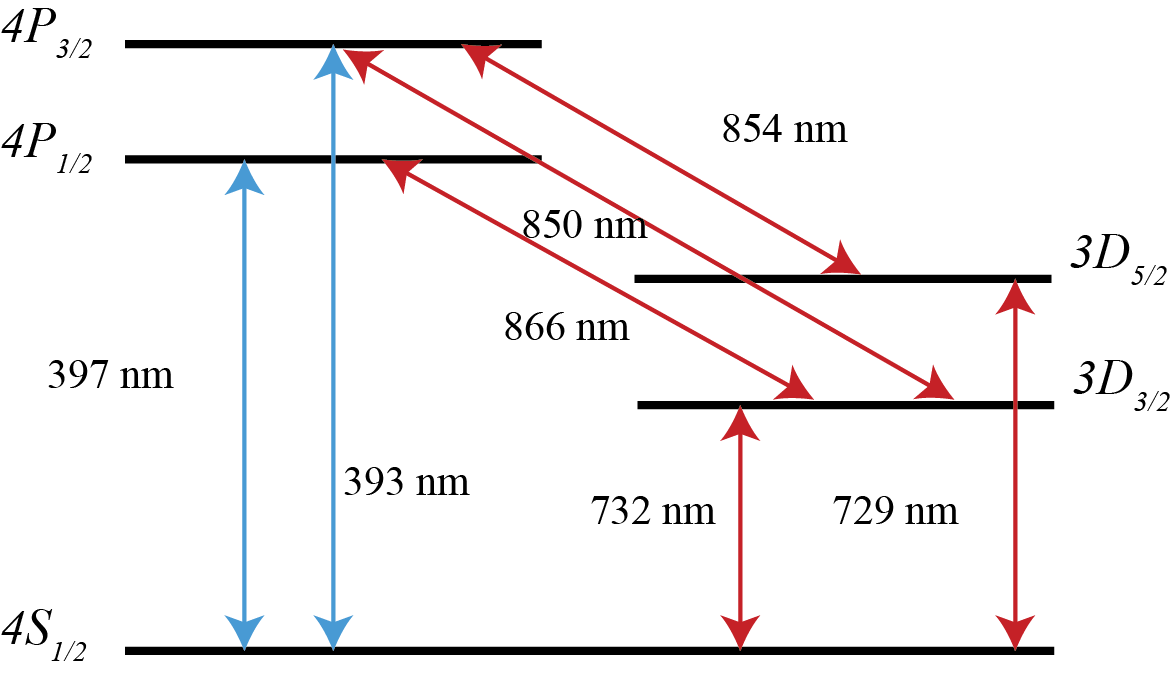
\includegraphics[width=.4\textwidth]{Chapters/Figures/calcium_levels_1-1.PNG}
\caption[Another short-form caption]{A figure included using the wrapfig environment}
\label{fig:anotherFigure}
\end{wrapfigure}
As an alternative to the ordinary figure environment, you might deem it desirable to tuck a figure in more closely amongst the text.  This has a separate environment known as \emph{wrapfig}.  Here we will include the same figure as above a second time, but this time using the \emph{wrapfig} environment.  This will insert the figure into your document with the text wrapping around the perimeter, rather than offsetting it into its own separate chunk of page, as above.    As before, we can use an automated reference to the figure using the \texttt{\textbackslash ref} tag; here we have figure~\ref{fig:anotherFigure}.  Working with the wrapfigure environment sometimes requires a little bit of massaging to ensure that everything lines up properly in your document, but with a small amount of work  you will find that you can get the text to box the figure quite nicely.

Here I have added a table, because tables are also useful. This table has nothing to do with the rest of the material in this thesis template, but you should probably only add relevant tables.
\begin{table}[tbh]
\begin{center}
%\caption[]{\em{Here we show the continuum sensitivity required per band.}}
\begin{tabular}{ccccccc}
\hline \noalign {\smallskip}
Name & SpT & Dist. & Age & 3$\sigma$ M$_{\rm dust}$ & 3$\sigma$ CO(3-2) limit & Disk indicator \\
 & & (pc) & (Myr) & limit (M$_{\oplus}$) &  (mJy km s$^{-1}$)\\
\hline \noalign {\smallskip}
J0226 & L0 & 46.5 & 45 & 0.01 & 24 & Pa$\beta$, IR\\
J0501 & M4.5 & 47.8 & 42 & 0.01 & 23 & H$\alpha$, IR\\
J1546 & M5 & 59.2 & 55 & 0.01 & 14 & HeI, [OI], H$\alpha$, IR\\
J0446 A/B & M6/M6 & 82.6/82.2 & 42 &  0.027 & 18 & H$\alpha$, IR\\
J0949 A/B & M4/M5 & 79.2/78.1 & 45 &  0.024 & 17 & H$\alpha$, IR\\
LDS 5606 A/B & M5/M5 & 84/84 & 30-44 & 0.027 & 19 & H$\alpha$, IR, UV\\
\hline \noalign {\smallskip}
\end{tabular}
\end{center}
\end{table}


